



\chapter{Implementação}
\label{implementacao}





Neste capítulo, são explicados os detalhes da implementação deste projeto, incluindo especificamente o projeto Django que inclui o sistema de informação com a aplicação web (\textit{frontend}/\textit{backend}) e a API REST. Para além disso, é descrita a implementação da simulação em \textit{hardware} para o cenário descrito no capítulo anterior bem como o sistema de videovigilância para deteção de intrusos. 

Segundo o ciclo de vida de um \textit{software}, estabelecido por \textit{Saini e Kaur}\cite{Saini2014} que se apresentou na secção \ref{method}, este capítulo irá incluir, em parte, a fase de \textit{designing} mas sobretudo a fase de \textit{coding}. 





\section{Sistema de informação}


Relativamente ao projeto Django, numa primeira fase procedeu-se à incorporação do \ac{SGBD} PostgreSQL através do psycopg2\footnote{\url{http://initd.org/psycopg/docs/}}. O psycopg2 consiste num adaptador entre o PostgreSQL com a linguagem de programação Python, que permite executar de forma eficiente qualquer \textit{script} em \ac{SQL}. É de notar que nesta fase inicial, se encontram instaladas algumas aplicações nativas do Django entre as quais, o  \texttt{django.contrib.auth} e  o \texttt{django.contrib.sessions}. Através delas é possível verificar o total funcionamento da base de dados uma vez que permitem a criação automática das tabelas associadas aos utilizadores, grupos, permissões e respetivos conteúdos, administração, sessões, entres outros. Estas tabelas são fundamentais ao bom funcionamento do sistema, sendo consideradas no modelo de dados descrito na secção \ref{modelocap}. 


Posteriormente, procedeu-se à criação dos diferentes \texttt{Models} conforme a nomenclatura apresentada nas tabelas \ref{tabeladb1} e \ref{tabeladb2} da secção \ref{modelocap}. O excerto de código seguinte pretende exemplificar a criação de um \texttt{Model} associado à tabela que representa a estrutura \acl{SM}, com o respetivo identificador e atributos.  Após a criação de cada \texttt{Model} procedeu-se à migração dos dados para o \ac{SGBD} onde foi possível verificar que as tabelas tinham sido criadas, através da utilização da ferramenta gráfica pgAdmin III. De modo a testar a estrutura criada, procedeu-se à introdução de dados através da zona administrativa do Django (figura \ref{admingdjango}). Através dos dados introduzidos e descrevendo um cenário realista foi possível validar a estrutura e proceder à implementação da aplicação \textit{web} e criação da \ac{API} \ac{REST}. 




\begin{lstlisting}[
language=Python,
showspaces=false,
basicstyle=\ttfamily,
numbers=left,
numberstyle=\tiny,
commentstyle=\color{gray},
basicstyle=\ttfamily\footnotesize
]
class SensorModule(models.Model):
	id = models.AutoField(primary_key=True)
	name = models.CharField(max_length=128)
	seding_time = models.IntegerField()
	status_sm = models.BooleanField(default=True)
	baterry_sm = models.IntegerField()
	localization_sm = models.CharField(max_length=128)
		
	def __str__(self):
		return "#"str(self.id) + " name_"+str(self.name)


\end{lstlisting}


\begin{figure}[!htb]
	\centering
	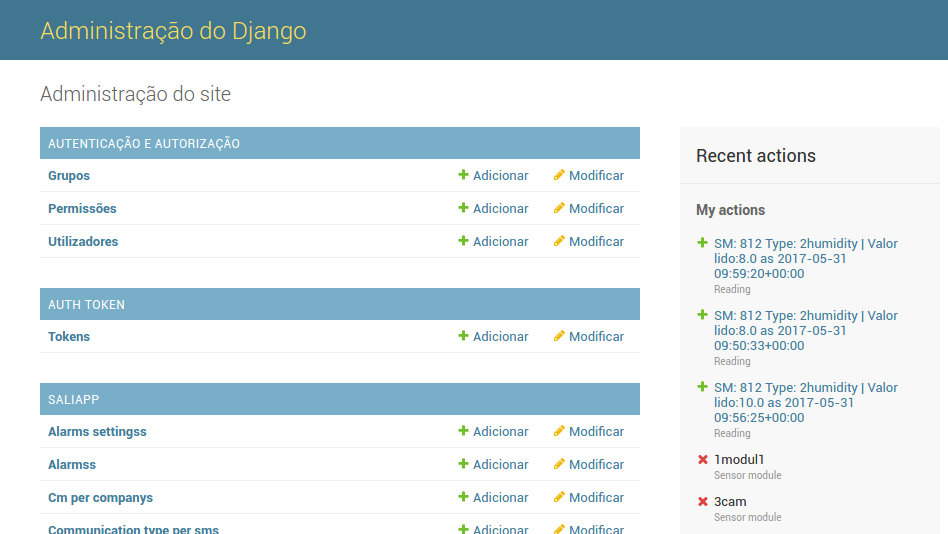
\includegraphics[scale=0.4]{prints-web/admindjango.png}
	\caption{Área administrativa da \textit{framework} Django }
	\label{admingdjango}
\end{figure}








\subsection{Sistema de registo e autenticação}

Primeiramente, procedeu-se à adaptação do \textit{template} AdminLTE de modo a criar as páginas de autenticação e registo dos utilizadores. Como vimos anteriormente, irão existir utilizadores distintos. Assim, de modo a identificá-los e a definir as suas permissões, houve necessidade de criar grupos específicos. Foram então criados dois grupos:  \textit{company}, que identifica uma empresa e \textit{general}, que identificada um utilizador comum. O administrador do sistema é um utilizador que tem o estado de \textit{superuser} ativo, isto é, possui todas as permissões sem que estas lhe sejam atribuídas explicitamente.


\begin{figure}[!htb]
	\centering
	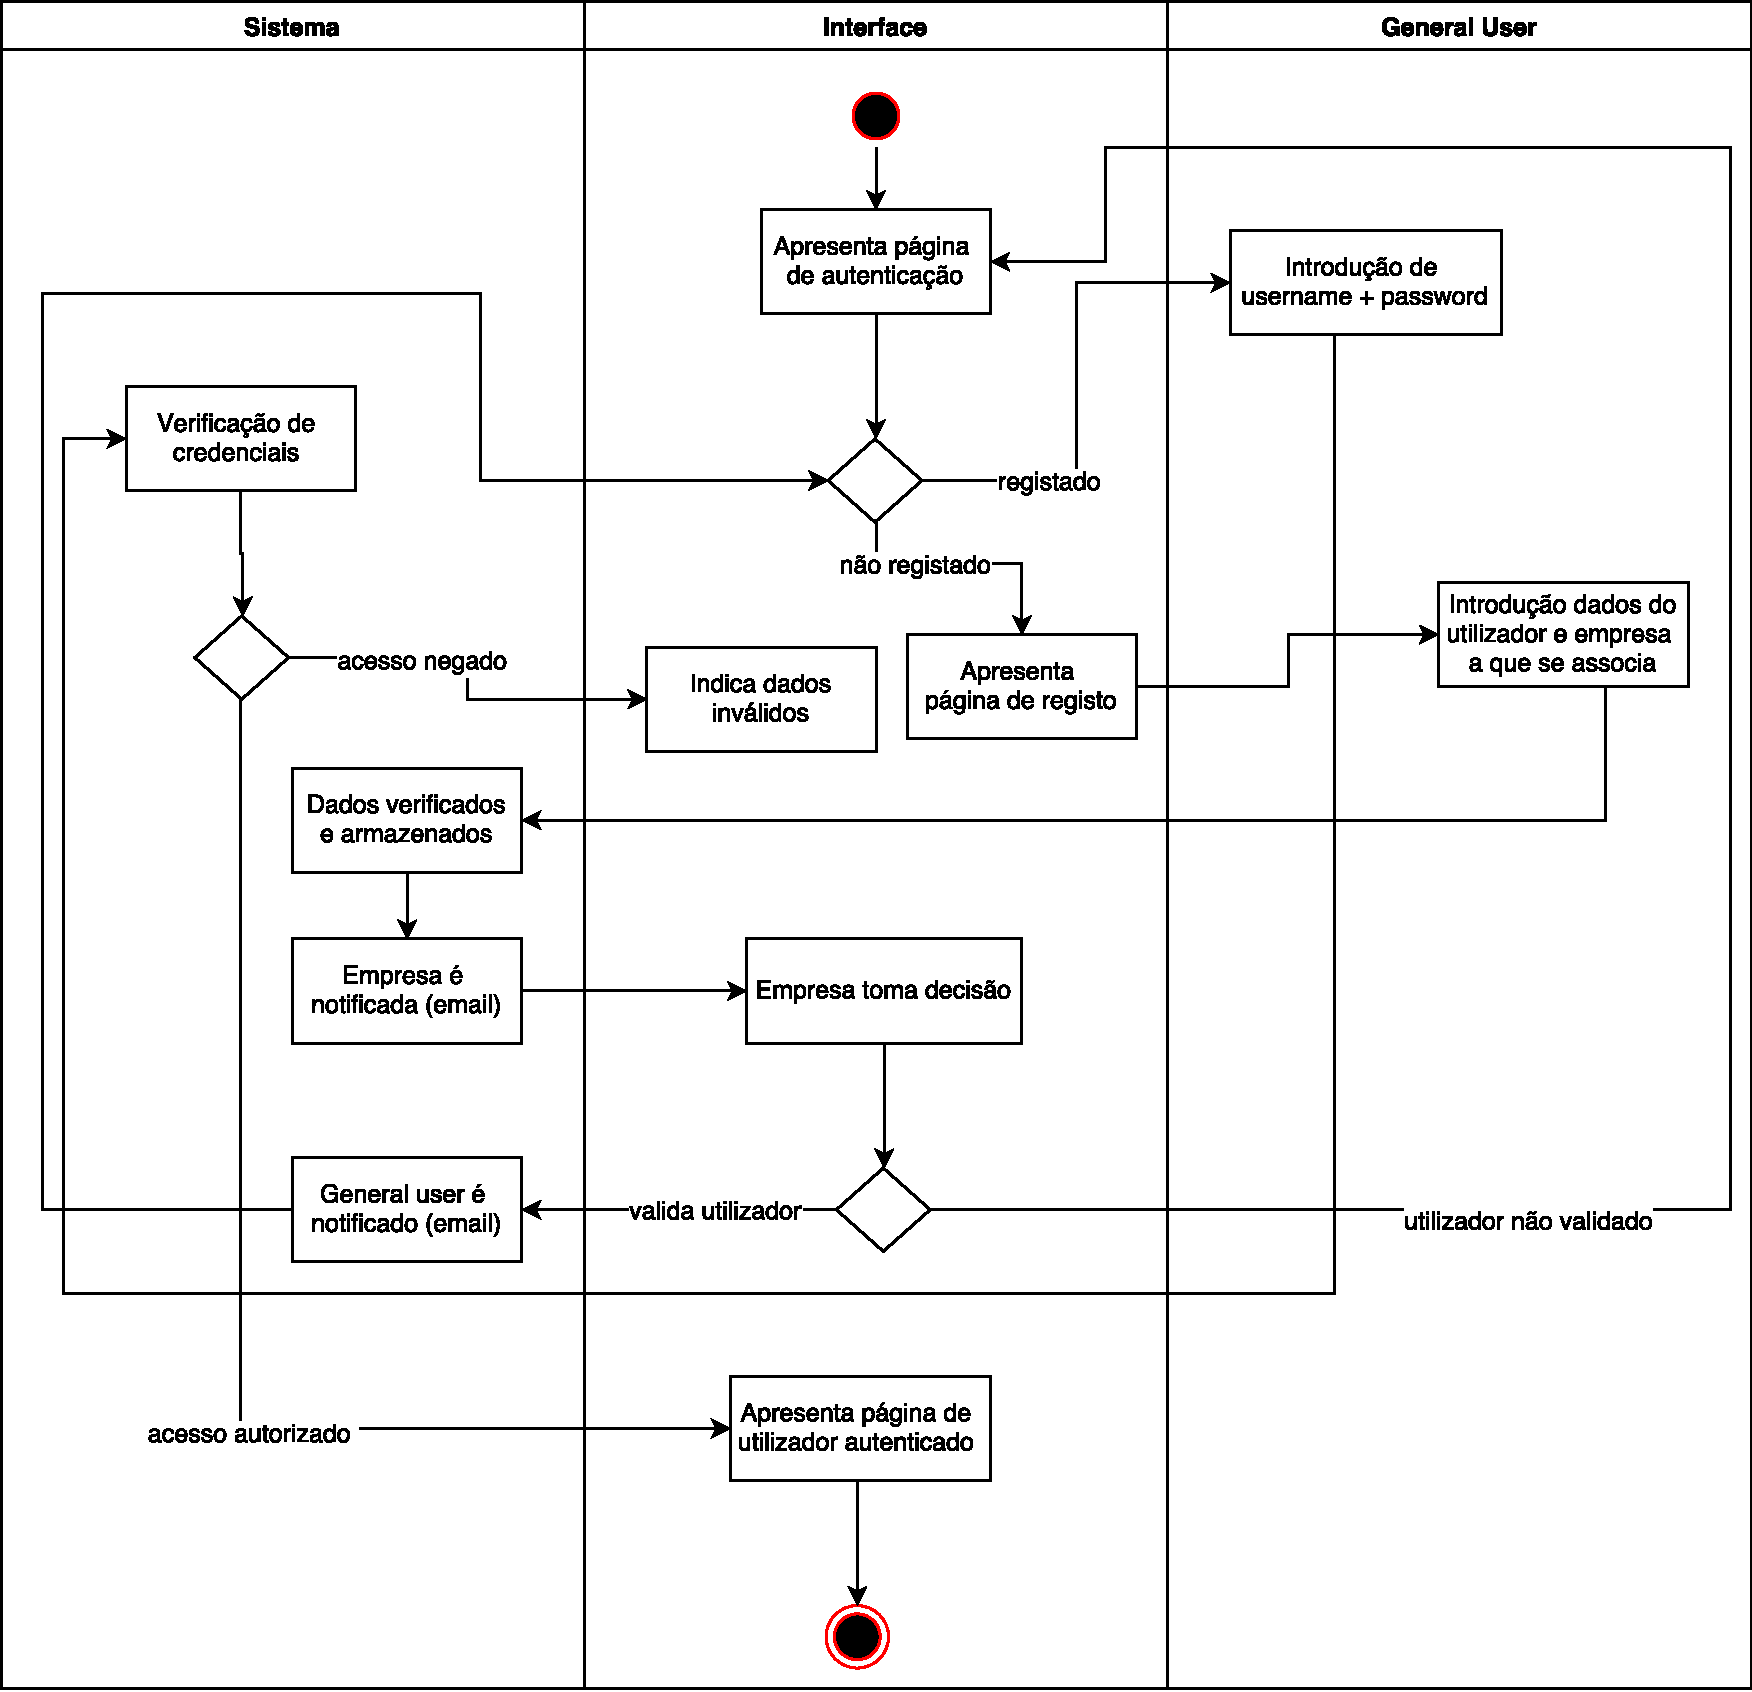
\includegraphics[width=\linewidth]{esquemas/activitydiagram-autenticacao.pdf}
	\caption{Diagrama de atividades do processo de registo e autenticação}
	\label{activt-autent}
\end{figure}


Como vimos anteriormente, o \textit{company user} apenas poderá ser adicionado ao sistema pelo admistrador, tendo este também permissões de gerir todos os utilizadores registados. Por outro lado, os \textit{company user} têm a possibilidade de validar os \textit{general user} que se associam à sua empresa, tendo posteriormente acesso aos dados/conteúdos desta. Após o registo de um novo \textit{general user} e a validação por parte do \textit{company user}, existem notificações que são enviadas via email. Estas mensagens são enviadas recorrendo ao método \texttt{send\_mail}\footnote{\url{https://docs.djangoproject.com/en/1.11/topics/email/}} existente nativamente no Django pelo pacote \texttt{django.core.mail}, sendo construido através do módulo \texttt{smtplib}\footnote{Módulo que define objetos para sessões \ac{SMTP} \url{https://docs.python.org/3/library/smtplib.html\#module-smtplib}}. Na figura \ref{activt-autent} apresenta-se o diagrama de atividades que ilustra o processo de registo de um \textit{general user} que envolve o utilizador responsável pela empresa (\textit{company user}). 








\subsection{Geração de alarmes}

No modelo de dados definido, cada sensor tem que ter obrigatoriamente associado a uma entrada na tabela \texttt{AlarmsSettings} que permite definir o valor máximo e mínimo para o qual são gerados alarmes bem como as mensagens de notificação enviadas ao utilizador. 

A geração de alarmes é condicionada pela comparação do valor lido pelos sensores com o valor máximo e mínimo definidos para o sensor em questão. Uma vez que é necessária esta verificação para cada leitura, criou-se um \textit{trigger} em \ac{SQL} que execute este procedimento, ao nível da \ac{SGBD} tornando o processo mais eficiente. Um \textit{trigger} permite que uma determinada sequência de comandos seja executada sempre que um determinado evento ocorra, neste caso uma adição. No Apêndice \ref{triggerSQLImpe} apresenta-se o \textit{stored procedure} (função) que implementa a sequência de comandos bem como a implementação do \textit{trigger} na linguagem \ac{SQL}. Na figura \ref{fluxoSP} encontra-se um diagrama de fluxo que permite ilustrar a lógica do \textit{stored procedure} implementado. 



\begin{figure}[!htb]
	\centering
	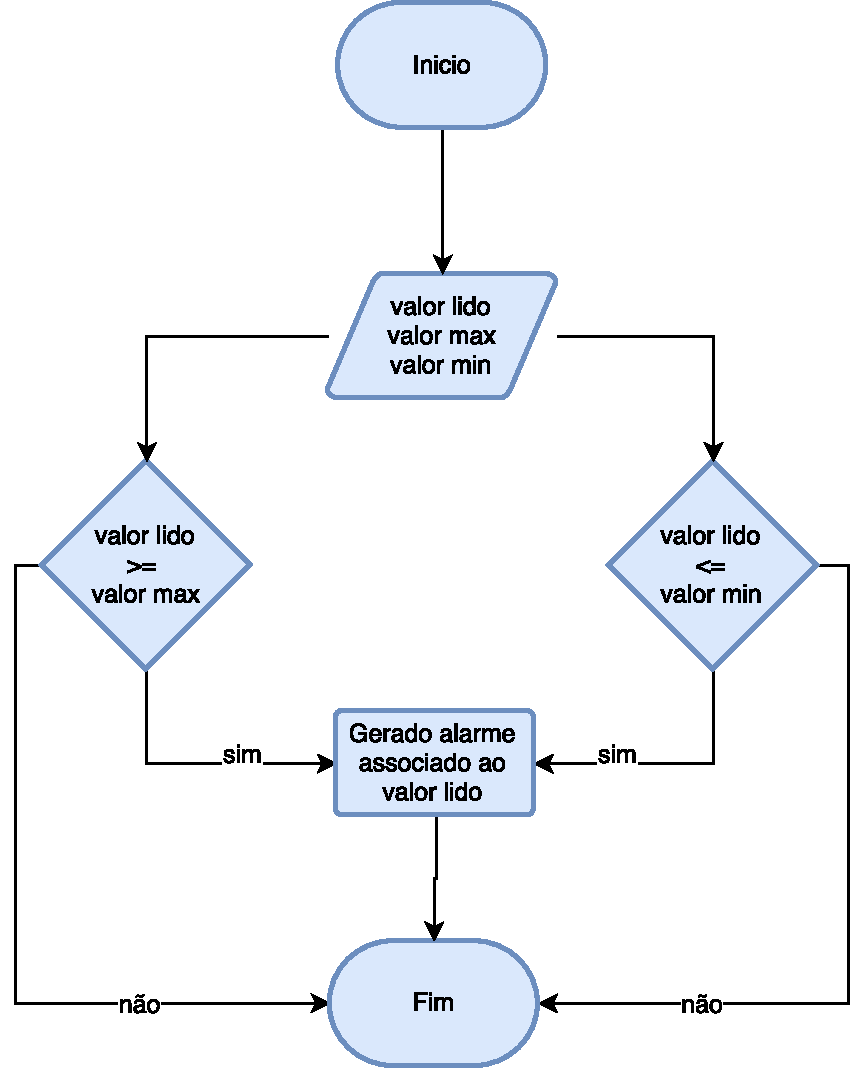
\includegraphics[scale=0.5]{esquemas/diagramafluxoalarms.pdf}
	\caption{Diagrama de fluxo para geração de alarmes}
	\label{fluxoSP}
\end{figure}



%\begin{itemize}
%	\item Análise do valor médio de cinco medições e respetivo desvio padrão 
%	\item Análise dos dados, também conhecida por data analist......... falta desenvolver data mining  
%\end{itemize}


O utilizador através da \textit{dashboard} e da aplicação \textit{mobile} poderá analisar os alarmes gerados bem como se os valores lidos pelos sensores se encontram dentro do intervalo previamente definidos. Para além disso, é apresentada a mensagem pré-definida (notificação) para que o utilizador possa tomar uma decisão.   



\newpage
\subsection{Visualização dos dados e cálculos estatísticos}

O cliente do sistema ao aceder à \textit{dashboard} e visualizar os detalhes de um determinado \acl{CM} ser-lhe-á apresentada uma lista de todos os \textit{Sensor Modules} que este possui. Juntamente com esta lista são apresentadas as caraterísticas principais de cada um, destacando os sensores existentes, o intervalo de tempo em que são enviados dados, a percentagem de bateria, as coordenadas da localização do módulo e os tipos de comunicação com o \acl{CM}. Complementarmente são apresentados quatro botões com icons ilustrativos que permitem realizar tarefas distintas.  

\begin{itemize}
	\item \faEdit \space (editar): possibilita editar as características enumeradas anteriormente para cada \acl{SM}. 
	\item \faTrash \space (remove): permite remover um determinado \acl{SM} de um \acl{CM}. 
	\item \faBarChart \faCogs \space (visualização gráfica e atuação remota): é possível visualizar graficamente os dados obtidos pelos diferentes sensores existentes num \acl{SM} bem como atuar remotamente num determinado atuador. 
	\item \faDatabase \space (visualização tabular): disponibilizada em vista tabular dos dados obtidos pelos sensores bem como a respetiva exportação para um ficheiro \ac{CSV}. 
\end{itemize}


Em ambas as visualizações anteriormente descritas é possível fazer uma filtragem por data para os dados obtidos dos sensores de cada \acl{SM}. Esta filtragem pode ser efetuada através de sete formas diferentes: do dia, do dia anterior, dos últimos sete dias, dos últimos trinta dias, deste mês, do último mês e selecionando a data de início e de fim especificamente. 


No que toca à visualização gráfica toda a representação foi concebida recorrendo à biblioteca ZingChart em \ac{JS}, sendo que toda a manipulação de dados é realizada a nível de \textit{backend} e posteriormente apresentada através dos \textit{templates} do Django. Esta biblioteca permite ainda que o cliente possa guardar os gráficos obtidos em formato de imagem (PNG, JPEG ou PDF).  A análise estatística para o intervalo de datas considerado permitirá ao cliente visualizar o valor máximo lido, o valor mínimo lido bem como o valor médio, sendo também todo o processamento realizado a nível de \textit{backend}. Para além disso, a página de visualização gráfica também possibilitará a ativação/desativação remota dos atuadores existentes no terreno. 


Por fim, relativamente à visualização tabular os dados são apresentados em três campos distintos que representam o tipo de sensor, data e hora da leitura, valor lido e a escala. A tabela contém paginação sendo possível escolher o número de entradas que serão apresentadas (10, 25, 50 ou 100). Complementarmente, existe uma caixa de texto que permite ao cliente pesquisar pelos campos apresentados. Para além disso é possível ordenar alfabeticamente ou numericamente esses campos (figura 6.17). O cliente também poderá exportar os dados apresentados num ficheiro do tipo \ac{CSV} com a estrutura apresentada na tabela \ref{exportcsv}. Para a implementação desta funcionalidade foram utilizados os métodos \texttt{writer} e \texttt{writerow()} disponíveis no pacote \texttt{csv} do Python.  


\begin{table}[h]
	\centering

	\begin{tabular}{|l|l|l|l|l|}
		\hline
		ID & Sensor type & Scale & Date time & Value \\ \hline
		579 & Water valve & 0/1 & 2017-05-31 09:30:14.762099+00:00 & 1 \\ \hline
		580 & Temperature & C & 2017-05-31 09:33:15.451236+00:00 & 25 \\ \hline
		581 & Water level & 0/1 & 2017-05-31 09:33:15.505198+00:00 & 1 \\ \hline
	\end{tabular}
	\caption{Estrutura do ficheiro do tipo \acs{CSV} possível de exportação}
	\label{exportcsv}
\end{table}




\subsection{API}


Tal como referido no capítulo anterior, para a implementação desta API do tipo REST foi utilizado o \textit{Django REST framework}. Para tal, instalou-se a aplicação \texttt{'rest\_framework'} no ficheiro de configuração do projeto Django, em \texttt{settings.py}. Para iniciar esta implementação procedeu-se à realização do \textit{quickstart} disponível no site oficial da \textit{framework}\cite{quickstart}. 

Primeiramente, procedeu-se à criação de um novo módulo \texttt{serializers.py} onde foram instanciadas todas as classes serializáveis\footnote{Consiste num processo de tradução de uma estruturas de dados ou de um objeto que pode ser armazenado (num arquivo ou \textit{buffer} de memória) e reconstruido posteriormente.  } para cada \texttt{Model} existente bem como  para os campos a considerar que possam ser usados na representação dos dados em formato \ac{JSON} ou \ac{XML}. De seguida, desenvolveu-se o módulo \texttt{apiViews.py} onde foram implementadas todas as classes baseadas na \texttt{APIView}. A classe \texttt{APIView} é uma subclasse da \texttt{View} (abordada no capítulo \ref{state}) tendo algumas diferenças: 

\begin{itemize}
	\item Na classe \texttt{View} são retornados objetos do tipo \texttt{HttpRequest} ou \texttt{HttpResponse}, enquanto que na \texttt{APIView} são objeto do tipo \texttt{Request} e \texttt{Response}; 
	\item A classe \texttt{APIView} permite a implementação dos seguintes métodos \ac{HTTP}: 	\texttt{get()}, \texttt{post()}, \texttt{put()} e \texttt{delete()}; 
	\item Através da classe  \texttt{APIView} podem ser implementadas várias políticas da \ac{API}. 
\end{itemize}

 
A título de exemplo, no excerto de código seguinte encontra-se a implementação do \textit{endpoint} \texttt{api/cm/\{pk\_or\_name\}} para o método GET. 

\begin{lstlisting}[
language=Python,
showspaces=false,
basicstyle=\ttfamily,
numbers=left,
numberstyle=\tiny,
commentstyle=\color{gray},
basicstyle=\ttfamily\footnotesize
]
#in serializers.py
class ControllerModuleSerializer(serializers.HyperlinkedModelSerializer):
	id_communication = CommunicationTypeSerializer()
	id_by_create = UserSerializer()

	class Meta:
		model = ControllerModule
		fields = ('id', 'name', 'id_communication', 'id_by_create', 'baterry_cm', 'status_cm', 'date_create','memory','localization_cm')

#in apiViews.py 
class ControllerModule_param(APIView):
	def get_object(self, pk_or_name):
		if pk_or_name.isdigit():
			try:
				return ControllerModule.objects.get(pk=pk_or_name)
			except ControllerModule.DoesNotExist:
				raise Http404
		else:
			try:
				return ControllerModule.objects.get(name__iexact=pk_or_name)
			except ControllerModule.DoesNotExist:
				raise Http404
	
	def get(self, request, pk_or_name, format=None):
		cm = self.get_object(pk_or_name)
		serializer = ControllerModuleSerializer(cm)
		return Response(serializer.data)

#in url.py
url(r'^api/cm/(?P<pk_or_name>[-\w]+)/$',views.ControllerModule_param.as_view()



\end{lstlisting}



Como descrito anteriormente, a autenticação desta API usa um método de autenticação via \textit{token}. Para tal, foi necessário a instalar a aplicação \texttt{'rest\_framework.authtoken'} que fornece a estrutura \texttt{Token}, possibilitando a criação e modificação do \textit{token} quando pretendido. Para que a autenticação seja possível é necessário incluir no módulo de configuração do Django o método pretendido, neste caso  \ \texttt{'rest\_framework.TokenAuthentication'}. Sempre que um utilizador é adicionado ao sistema também o respetivo \textit{token} é gerado. Para além disso, o utilizador poderá renovar o \textit{token} sempre que pretendido. No anexo \ref{espcifAPIREST} encontram-se as especificações de cada \textit{endpoint} existente nesta API REST.






\subsection{Documentação da API}

Para a utilização da documentação interativa da API REST foi utilizada a ferramenta Swagger. Para a sua utilização foi necessário incluir a aplicação \texttt{'rest\_framework\_swagger'} no ficheiro \texttt{settings.py} do Django e seguindamente definir o \ac{URL} que lhe permitirá o acesso. Na figura \ref{docapi} encontra-se um exemplo ao consultar a documentação desta API. 

\newpage

\begin{figure}[h]
	\centering
	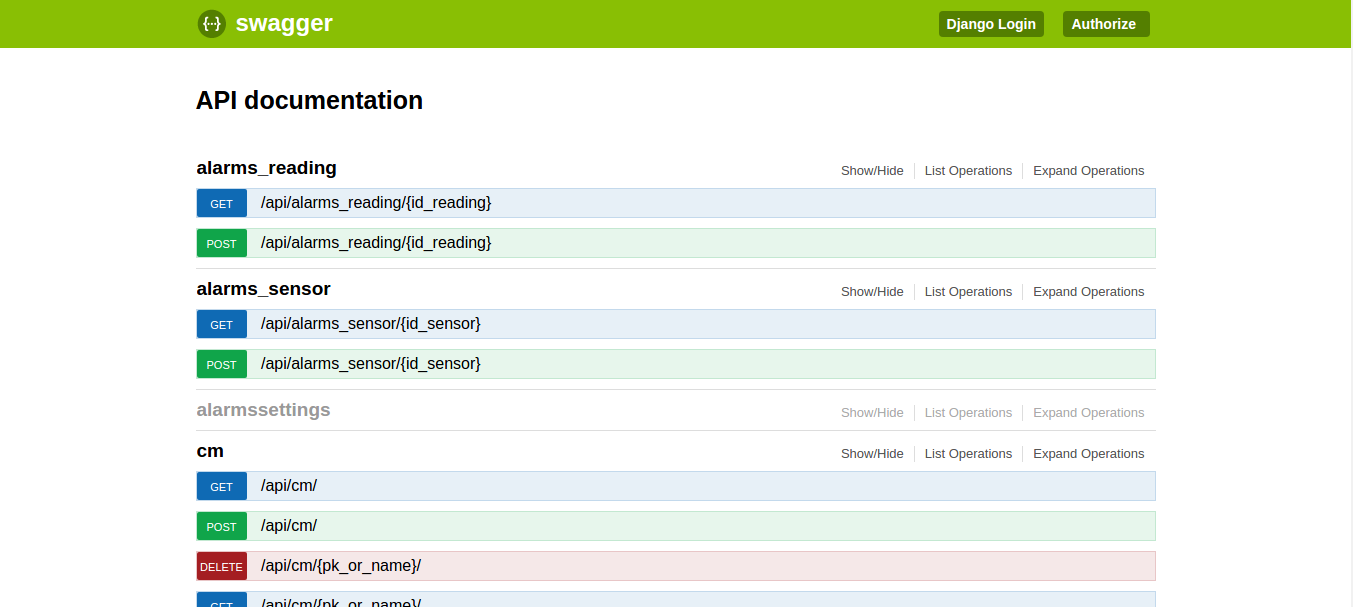
\includegraphics[width=0.91\linewidth]{prints-web/api-doc.png}
	\caption{Documentação da API REST com a ferramenta Swagger}
	\label{docapi}
\end{figure}


\subsection{Aplicação \textit{web}}

Ao utilizador da \textit{dashboard}, após fazer a autenticação, ser-lhe-ão apresentados todos os \textit{Controller Modules} a que tem acesso bem como as seguintes informações para cada um:


\begin{itemize}
	\item Mapa onde é possível localizar todos os módulos associados a um \acl{CM}; 
	
	\item Alarmes gerados pelos sensores que os \textit{Sensor Modules} possuem e respetivas notificações; 
	
	\item Últimos valores lidos pelo sensores dos \textit{Sensor Modules}.
\end{itemize} 



Cada um dos mapas interativos permitirá localizar o \acl{CM} bem como os \textit{Sensor Modules} a si associados, sendo estes identificados por marcadores\footnote{Um marcador identifica uma localização no mapa. \\ \url{https://developers.google.com/maps/documentation/javascript/markers?hl=pt-br}} de diferentes cores - no caso do \acl{CM}, a vermelho e nos \textit{Sensor Modules}, a azul. A implementação destes mapas recorre à \ac{API} do Google Maps em \ac{JS}, permitindo receber a localização dos módulos em coordenadas \ac{GPS}. Ao clicar sob um determinado marcador este irá direcionar o utilizador para a página de detalhes do módulo em questão. 


Quando surge um  alarme, o utilizador poderá verificar o motivo pelo qual este foi gerado, consultar a mensagem resultante bem como o valor lido, tendo ainda a possibilidade eliminar o alarme para que este não seja mais apresentado em destaque. Para além disso, o utilizador ao aceder à \textit{dashboard} ser-lhe-ão apresentados os últimos valores lidos por cada sensor, distribuídos por cada \acl{SM}. Adicionalmente, na página principal da plataforma são apresentados alguns valores estatísticos da mesma: número de utilizadores registados, número de \textit{Sensor Modules}, número de \textit{Controller Modules} e número de leituras que já foram recolhidas pelos diferentes sensores. 


A interface gráfica da plataforma permite ainda que o utilizador comum possa: 

\begin{itemize}
	\item Aceder à página de perfil possibilitando ao utilizador alterar as suas informações básicas e redefinir a sua \textit{password}. Para além disso, também pode consultar o \textit{token} de autenticação para a  \ac{API}; 
	
	\item Consultar, adicionar ou editar os detalhes dos \textit{Controller Modules} e dos \textit{Sensor Modules}; 
	
	\item Adicionar e consultar dos tipos de sensores e comunicações existentes; 
	
	\item Alterar o avatar existente através da ferramenta \textit{Gravatar} disponível em \url{http://pt.gravatar.com/}. 
\end{itemize}






Sempre que o utilizador executa uma determinada ação na plataforma este é notificado informando-o se a ação foi bem sucedida ou não. A implementação deste mecanismo recorre à estrutura de mensagens\footnote{\url{https://docs.djangoproject.com/en/1.11/ref/contrib/messages/}} do Django, também conhecida por mensagens de \textit{flash}. 




\subsection{\textit{Deploy} do projecto}

Para implementar o projeto Django juntamente com o servidor \textit{web} Apache 2.0 num \ac{VPS} Linux (Ubuntu 14.X), foram seguidos os seguintes passos: 


%https://jee-appy.blogspot.com.tr/2015/04/deploy-django-project-on-apache-using.html




\begin{enumerate}
	\item Instalação do Python na versão 2.7 bem como pip\footnote{Sistema de gestão de pacotes usado para instalar e gerir pacotes de software escritos na linguagem Python.} e respetivo \textit{upgrade} para a versão mais recente
	
	\texttt{sudo apt-get install python-pip python-dev build-essential}
	
	\texttt{sudo pip install --upgrade pip}
	
	
	\item Instalação do PostgreSQL na ultima versão e criação de uma base de dados com o nome salibd
	
	
	\texttt{sudo apt-get install postgresql postgresql-contrib}

	\texttt{createdb salibd}	
	
	
	\item Instalação do apache2 e do mod\_wsgi que fará a ligação do projeto Python com o servidor apache. Seguidamente dar reset ao apache2.
	
	\texttt{sudo apt-get install apache2}
	
	\texttt{sudo apt-get install libapache2-mod-wsgi}
	
	
	\item Configuração do virtualenv\footnote{\url{https://virtualenv.pypa.io/en/stable/}}, que consiste numa ferramenta para criar ambientes Python isolados. Por outro lado o virtualenvwrapper\footnote{\url{https://virtualenvwrapper.readthedocs.io/en/latest/}} permite uma fácil gestão do virtualenv, sendo que ao instalá-lo através do pip o virtualenv será instalado automaticamente. 
	
	
	\texttt{pip install virtualenvwrapper}
	
	 
	\item Criar um ambiente virtual (virtualenv) para o projeto. Para a criação foi utilizada a opção \texttt{--system-site-packages} uma vez que a nossa aplicação terá que aceder a recursos fora do ambiente virtual, neste caso o PostgreSQL. 
	
	\texttt{mkvirtualenv exampleenv --system-site-packages}
	
	
	\item Adicionar o projeto e instalar dependências. Primeiramente, foi necessário ativar o virtualenv. Seguidamente procedeu-se à instalação do Django e instalação dos requisitos da aplicação (através do ficheiro requirements.txt disponibilizado pelo IDE). 
	
	\texttt{workon exampleenv}
	
	\texttt{pip install Django}
	
	\texttt{cd /var/www}
	
	\texttt{git clone https://github.com/ruipoliveira/ThesisSalicornia-web.git}
	
	\texttt{pip install -r requirements.txt}
	
	

	

	\item Criação do virtual host. Terá que estar no directório \texttt{/etc/apache2/sites-available/} e criar um ficheiro \texttt{.conf} com o seguinte conteúdo. 
	
	\begin{lstlisting}[
	showspaces=false,
	basicstyle=\ttfamily,
	numbers=left,
	numberstyle=\tiny,
	commentstyle=\color{gray},
	basicstyle=\ttfamily\footnotesize
	]
	<VirtualHost *:80>
	ServerAdmin webmaster@mydomain.com
	ServerName 192.168.160.20
	ServerAlias http://192.168.160.20
	WSGIScriptAlias / /var/www/example.wsgi
	
	Alias /static/ /var/www/ThesisSalicornia-web/saliDashboard/saliapp/static/
		<Location "/static/">
			Options -Indexes
		</Location> 
	
	<Directory /var/www/ThesisSalicornia-web/saliDashboard>
	Order deny,allow    
	Allow from all
	</Directory>
	</VirtualHost>
	\end{lstlisting}
	
	Por fim, é necessário ativar esta configuração através do comando:
	
	\texttt{a2ensite example.conf}
	
	
	\item Criação do ficheiro wsgi no directório \texttt{/var/www/}
	
	\begin{lstlisting}[
	language=Python,
	showspaces=false,
	basicstyle=\ttfamily,
	numbers=left,
	numberstyle=\tiny,
	commentstyle=\color{gray},
	basicstyle=\ttfamily\footnotesize
	]
	#file name 'example.wsgi'
	import os
	import sys
	import site
	# Add the site-packages of the chosen virtualenv to work with
	site.addsitedir('/var/www/.virtualenvs/exampleenv/local/lib/python2.7/site-packages')
	# Add the app's directory to the PYTHONPATH
	sys.path.append('/var/www/ThesisSalicornia-web/saliDashboard')
	sys.path.append('/var/www/ThesisSalicornia-web/saliDashboard/saliDashboard')
	os.environ['DJANGO_SETTINGS_MODULE'] = 'saliDashboard.settings'
	# Activate your virtual env
	activate_env=os.path.expanduser("/var/www/.virtualenvs/exampleenv/bin/activate_this.py")
	execfile(activate_env, dict(__file__=activate_env))
	from django.core.wsgi import get_wsgi_application
	application = get_wsgi_application()\end{lstlisting}
	
	
	\item Sincronizar a base de dados através do comando: 
	
	\texttt{python manage.py migrate}
	
	 
	 
	 
\end{enumerate}




%\subsection{Aplicação mobile}








\section{Simulação em \textit{hardware}}

Nesta secção explica-se a implementação a nível de \textit{software} no contexto desta simulação para cada um dos microcontroladores. 


\subsection{Arduino Nano}
\label{arduinonanoard}

No que diz respeito ao Arduino Nano (\acl{SM}), numa fase inicial,  fez-se a ligação dos diversos componentes  apresentados na secção \ref{arq-hardw} a uma placa branca (\textit{breadboard}) tal como apresentado no Anexo \ref{interlapd}. Para auxiliar o desenvolvimento do \textit{software} foi utilizada a versão 1.8.1 do \ac{IDE} do próprio Arduino\footnote{\url{https://www.arduino.cc/en/Main/Software}}. Seguidamente apresenta-se a implementação necessária a nível de sensores e de comunicação. 


Foram desenvolvidos os seguintes métodos que permitem aceder aos valores lidos de cada um dos sensores. Para além disso, foi criado um método que permite alterar o estado de ativação do \ac{LED}, possibilitando a simulação do estado da válvula para transferência de águas. 

\begin{itemize}
	\item \texttt{int readTemperature(int port)}: é efetuada uma leitura no porto analógico através do método \texttt{analogRead} e seguidamente realizada uma conversão para ºC (graus Celsius);
	
	\item \texttt{long readLuminosity(int port)}: é efetuada uma leitura ao porto analógico e posteriormente é realizada uma conversão para percentagem (\%); 
	
	\item \texttt{int readWaterValve(int port)}: é efetuada uma leitura no porto digital através do método \texttt{digitalRead} disponibilizado pelo Arduino.
	
	\item \texttt{int readWaterLevel(int port)}: é realizada uma leitura no porto digital através do método \texttt{digitalRead}.
	
	
	\item \texttt{void setWaterValve(int port, int state)}: se a variável \texttt{state} for 1 então o porto é colocado a \texttt{HIGH} (1) através do método \texttt{digitalWrite}, caso contrário é colocado a \texttt{LOW} (0)
	
\end{itemize}

Inicialmente procedeu-se à leitura de cada sensor de forma individual de modo a garantir o seu total funcionamento. Sempre que é enviado um pedido de leitura dos sensores pelo \acl{CM} os valores são enviados no formato apresentado em \ref{eq:someequation}.

\begin{equation} 
\label{eq:someequation}
\texttt{<temperatura>;<nível\_água>;<luminosidade>;<estado\_válvula>}
\end{equation}



Numa primeira fase, procedeu-se à comunicação entre o \acl{SM} e \acl{CM} através de porta série. Seguidamente, incorporou-se o módulo Bluetooth de modo a tornar os dois módulos independentes. Foi utilizado o  \textit{package} \texttt{SoftwareSerial.h} disponibilizado pelo Arduino, que permite interagir facilmente com o módulo de comunicação utilizado. Posteriormente, decidiu-se quais os \textit{inputs} que o Arduino iria receber e que ações iria executar, concluindo-se que podiam ser recebidos valores entre 0 e 2. 


\begin{itemize}
	\item \textbf{0}: ativação do \ac{LED} (válvula para transferência de água); 
	\item \textbf{1}: desativação do \ac{LED} (válvula para transferência de água); 
	\item \textbf{2}: requisitar dados obtidos pelos sensores existentes no formato definido em \ref{eq:someequation}. 
\end{itemize}

Antes de proceder à implementação de envio e receção de dados por Bluetooth no Raspberry Pi 3, testou-se esta funcionalidade isoladamente. Para isso, utilizou-se uma aplicação existente na \textit{Play Store} denominada  de \textit{Bluetooth Terminal HC-05}\footnote{\url{https://play.google.com/store/apps/details?id=project.bluetoothterminal}}, que permitiu facilmente validar este mecanismo. Os resultados deste teste funcional serão apresentados no próximo capítulo. 



\subsection{Raspberry Pi 3}

Nesta simulação, o \acl{CM} recebe apenas os dados adquiridos por um \acl{SM}, e envia as ações que este terá que executar.  Para a comunicação entre os dois módulos, foi utilizado o módulo interno Bluetooth 4.1 disponível no \textit{hardware} do Raspberry Pi 3. De modo a conseguir receber os dados adquiridos e enviá-los para o servidor através da \ac{API}, desenvolveu-se um \textit{script} em Python que permite o seguinte: 


\begin{enumerate}
	\item Verificação dos dispositivos Bluetooth disponíveis. Para aceder a este recurso, foi utilizada uma extensão do Python denominada de \textit{pybluez}\footnote{\url{https://github.com/karulis/pybluez}}. 
	
	
	\item Estabelecer uma ligação com módulo HC-06 através de um \textit{socket} de comunicação (variável global na figura \ref{threadscript}). Para tal, foi utilizado o \textit{package} \texttt{socket} disponibilizado pelo Python.
	
	\item Foram criados dois \textit{threads} que permitem realizar funcionalidades distintas (figura \ref{threadscript}): 
	
	\begin{itemize}
		\item \textbf{Controlar estado da válvula}: permite aceder à \ac{API} de modo a verificar o estado do \ac{LED}  (válvula de admissão) e atualizá-lo sempre que necessário no \acl{SM}, através do método \texttt{send()}. No caso de ser enviado o dígito '1' o \ac{LED} será ligado (válvula aberta), enquanto que se for enviado o dígito '0' o  \ac{LED} será desligado (válvula fechada). 
		
		\item \textbf{Receção de dados}: no caso de ser enviado o  dígito '2', o \textit{socket} ficará a aguardar a receção dos dados lidos pelos sensores no formato definido, utilizando para isso o método \texttt{recv()}. Após a receção dos dados, é efetuado algum processamento para que estes possam ser enviados para o servidor através da \ac{API} REST. Os dados são enviados a um intervalo (\textit{seding time}) igual  ao definido pelo utilizador na \textit{dashboard}.
		
		
	\end{itemize}
	
	

\end{enumerate}





\begin{figure}[h]
	\centering
	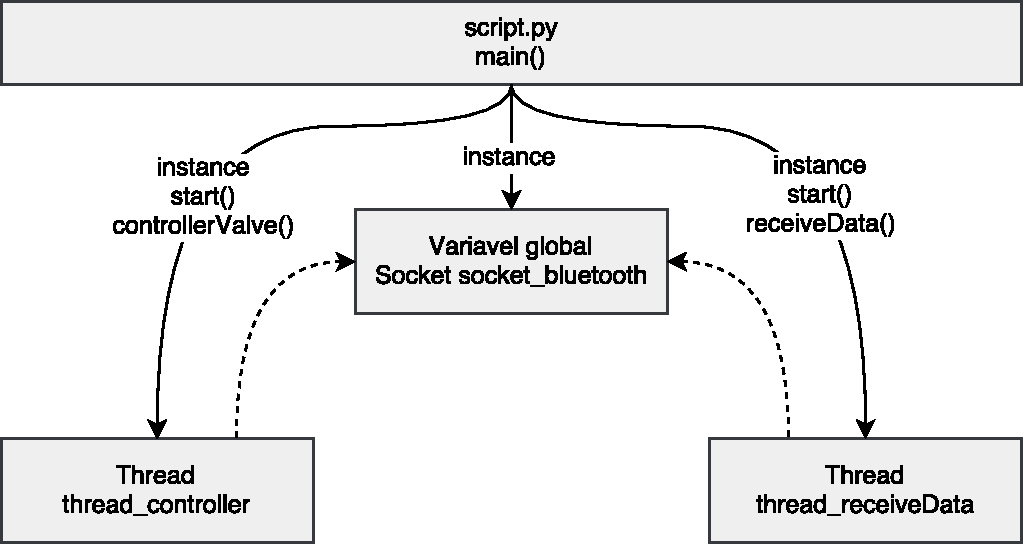
\includegraphics[width=0.67\linewidth]{esquemas/threads-python-script.pdf}
	\caption{Lógica de implementação do \textit{script} para o \acl{CM} }
	\label{threadscript}
\end{figure}










%>1 fase testar coneccao arduino to rasp via porta serie; foi criado um script em python para processar info e enviar para o servidor através da API 

%>2 fase : necessidade de tornar um módulo isolado sem necessidade de fio; foi testado um modulo wifi e bluetooth; 

%>neste contexto modulo wifi nao!... pretende-se que os sensor moduels sejam de baixo custo e low power. foi utilizado um modulo bluetooth; foi testada a conexao da comm bluetooth através de uma client disponveil na google play bluetooth terminal HC-05 


%>  pq nao foi usado um sensor de salinidade? nao havia orçamento.. 









\section{Sistema de videovigilância}


Tal como descrito na secção \ref{videoviarqut}, foram utilizadas as ferramentas FFmpeg e raspivid para envio de vídeo sem qualquer tipo de processamento para o servidor \ac{RTMP} do Youtube. Para testar a funcionalidade, foi executado o seguinte comando no terminal do Raspberry Pi 3, sendo possível observar o resultado na conta do Youtube.


\begin{lstlisting}[
language=Python,
showspaces=false,
basicstyle=\ttfamily,
numbers=left,
numberstyle=\tiny,
commentstyle=\color{gray},
basicstyle=\ttfamily\footnotesize]
raspivid -o - -t 0 -vf -hf -fps 30 -b 6000000 | ffmpeg -re -ar 44100 -ac 2 -acodec pcm_s16le -f s16le -ac 2 -i /dev/zero -f h264 -i - -vcodec copy -acodec aac -ab 128k -g 50 -strict experimental -f flv rtmp://a.rtmp.youtube.com/live2/ux4a-v8x7-3yws-635b

\end{lstlisting}






Seguidamente, são descritos alguns dos parâmetros mais importantes presentes no comando anterior\cite{streamlive}. 

\begin{itemize}
	\item \texttt{-o -}: grava o vídeo para que possa ser utilizado pelo FFmpeg; 
	
	\item \texttt{-t 0}: grava e transmite o vídeo até que seja parado manualmente; 
	
	\item \texttt{-vf -hf}: inverte a imagem (horizontal/vertical) para permitir uma correta visualização; 
	
	\item \texttt{-fps 30 }: define o numero de frames por segundo, neste caso 30. 
	
	\item \texttt{-ar 44100 -ac 2 -acodec pcm\_s16le -f s16le -ac 2 -i /dev/zero}: adiciona um canal de áudio preenchido a zeros, uma vez que o YouTube rejeita fluxos sem um canal de áudio; 
	
	\item \texttt{-f h264}: diz ao FFmpeg que irá receber entrada h264 ( padrão para compressão de vídeo). 
	
\end{itemize}






Para além do descrito anteriormente, foi criado um \textit{script} em python que permite a aquisição de imagem proveniente do Raspberry Pi através do package \texttt{picamera}\footnote{\url{http://picamera.readthedocs.io/en/release-1.13/}}. Este pacote, fornece  uma interface em Python (disponível para qualquer versão) para o módulo de câmara Raspberry Pi, permitindo uma fácil interação entre a aquisição da imagem e respetivo processamento.
Seguidamente será explicada a utilização de um algoritmo de deteção de intrusos disponibilizado pelo OpenCV. 


 


\subsection{Utilização do algoritmo de deteção de intrusos}
\label{algdetecao}
% artigo http://lear.inrialpes.fr/people/triggs/pubs/Dalal-cvpr05.pdf


Para a implementação do algoritmo de deteção de intrusos estudou-se o módulo \linebreak \texttt{peopledetect.py}\footnote{\url{https://github.com/npinto/opencv/blob/master/samples/python2/peopledetect.py}} disponível no repositório github do OpenCV. Este algoritmo permite detetar pessoas recorrendo a algoritmos específicos do OpenCV já treinados para o efeito, que serão descritos seguidamente. Complementarmente, foi analisado um artigo\cite{Dalal} que permitiu entender melhor a implementação apresentada, evidenciando o processo de deteção de características, algoritmos de treino (neste caso \ac{SVM}) e respetivos testes. No excerto de código seguinte encontra-se a implementação base fornecida pelo OpenCV para deteção de pessoas, que seguidamente será descrita. 

\begin{lstlisting}[
language=Python,
showspaces=false,
basicstyle=\ttfamily,
numbers=left,
numberstyle=\tiny,
commentstyle=\color{gray},
basicstyle=\ttfamily\footnotesize
]
hog = cv2.HOGDescriptor()
hog.setSVMDetector(cv2.HOGDescriptor_getDefaultPeopleDetector())

(rects, weights) = hog.detectMultiScale(img, winStride=(8,8), 
	padding=(32,32), scale=1.05)
\end{lstlisting}
	

\begin{itemize}
	\item \texttt{HOGDescriptor()}: esta classe implementa um histograma de gradientes orientados\cite{Dalal} que tem como objetivo a deteção de objetos; 
	
	\item \texttt{setSVMDetector()}: permite definir os coeficientes para um  classificador \ac{SVM} linear. O \ac{SVM} é um algoritmo de \textit{machine learning} usado para classificação e análise de regressões; 
	
	
	\item \texttt{getDefaultPeopleDetector()}: retorna um classificador pré-treinado para deteção de pessoas (para tamanho de janela padrão)\cite{featuredetection}; 
	
	
	\item \texttt{detectMultiScale()}: permite detetar objetos de diferentes tamanhos. Este método possui vários parâmetros que permitem ajustar o tamanho de deteção de um determinado objeto, como por exemplo o \texttt{winStride}, \texttt{padding} ou a \texttt{scale}; 
	
\begin{itemize}
	\item \texttt{winStride}: define o "tamanho do passo" na posição x e y de uma janela deslizante (figura \ref{winStride}). Este parâmetro é opcional;
	 
	\item \texttt{padding}: consiste num tuplo que indica o número de pixels, na direção x e y, tal como o \texttt{winStride}. Os valores típicos são (8, 8),  (16, 16), (24, 24) e (32, 32). É um parâmetro opcional que  define o preenchimento; 
	
	\item \texttt{scale}: este parâmetro controla o fator com que a imagem é redimensionada em cada camada da pirâmide de imagens (figura \ref{scale}), influenciando o número de níveis existentes. É um parâmetro opcional. 

\end{itemize}
	
	 %% http://www.pyimagesearch.com/2015/11/16/hog-detectmultiscale-parameters-explained/
	 
\end{itemize}



O algoritmo apresentado permite a deteção de intrusos (humanos), quando estes surgem em vídeos ou imagens. Pretende-se incorporar este algoritmo no sistema de videovigilância (Youtube Live), possibilitando a deteção de indivíduos quando estes são capturados pela câmara, gerando alarmes para a plataforma. Para incorporar o algoritmo apresentado com o Youtube Live é necessário entender o mecanismo de \textit{streaming} disponibilizado pela \ac{API} do YouTube Live Streaming\footnote{\url{https://developers.google.com/youtube/v3/live/getting-started}}.  


\newpage

\begin{figure}[h]
	\centering
	\begin{minipage}[b]{0.49\textwidth}
		\centering
		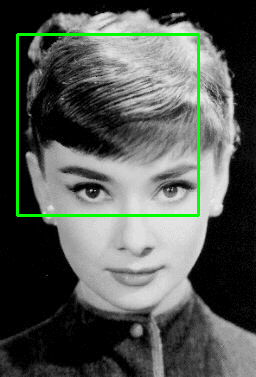
\includegraphics[width=0.4\textwidth]{img/sliding_window_example-11.png}
		\caption{Exemplo da aplicação do parâmetro \texttt{winStride} }
		\label{winStride}
	\end{minipage}
	\hfill
	\begin{minipage}[b]{0.49\textwidth}
		\centering
		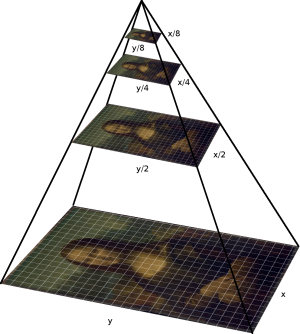
\includegraphics[width=0.5\textwidth]{img/pyramid.png}
		\caption{Pirâmide de imagens para diferentes \texttt{scale}}
		\label{scale}
	\end{minipage}
	
\end{figure}






Como vimos anteriormente, existem vários parâmetros para o método \linebreak \texttt{detectMultiScale()}, que permitem ajustar o tamanho da deteção. Dependendo da disposição exata da câmara, é possível ajustar estes parâmetros permitindo uma deteção o mais eficaz possível. No próximo capítulo serão apresentados alguns exemplos em que é possível testar o algoritmo apresentado.  










%Deteção de intrusos: http://www.pyimagesearch.com/2015/11/09/pedestrian-detection-opencv/



%versão simplificada: http://www.pyimagesearch.com/2015/02/16/faster-non-maximum-suppression-python/



%Servidor em falsk 


%deploy  https://iotbytes.wordpress.com/python-flask-web-application-on-raspberry-pi-with-nginx-and-uwsgi/



%Dataset: %http://www.robots.ox.ac.uk/ActiveVision/Research/Projects/2009bbenfold_headpose/project.html






\iffalse


\subsection{Testes}

Pretende-se instalar uma câmara na quinta onde se produz salicornia, de modo a detectar grande parte da área existente, sobretudo onde existe os módulos sensoriais mas também algumas máquinas utilizadas no cultivo desta especie. Para tal, tenciona-se colocar uma câmara, numa primeira fase uma \textit{Raspberry Pi camera module}, mas posteriormente poderá ser substituída por uma câmara IP de maior qualidade. Esta câmara irá coloca-se no topo de um armazém existente virada para o centro da quinta a aproximadamente 3 metros de altura. 

Com o objetivo de determinar quais os valores a atribuir aos parâmetros \texttt{winStride}, \texttt{padding} e \texttt{scale} foram realizados alguns testes com algumas imagens de um dataset onde seja possível detetar pessoas assumindo a mesma perspetiva, isto é, mesma altura e ângulo.  

Foram considerados quatro frames de um dataset disponibilizado pela Universidade de Oxford utilizado para diferentes estudos a nível do desempenho em processamento de imagem envolvendo sistemas de videovigilância, mais precisamente para detecção e tracking de pessoas\cite{imagProccdata}. O vídeo disponibilizado chama-se \texttt{TownCentreXVID.avi}. 

Os resultados obtidos, isto é o tempo de processamento, numero de pessoas detetadas bem como as imagens consideradas encontram-se no anexo X. Foram considerados os seguintes valores possíveis para os parâmetros estudos: 

\begin{itemize}
	\item \texttt{winStride}: (2, 2), (4, 4), (8, 8)
	
	\item \texttt{padding}: (8,8), (16, 16), (24, 24)
	
	\item \texttt{scale}: 0.5, 1.0, 1.5 
\end{itemize}


\subsection{Implementação}


Após concluir quais os melhores valores a utilizar como parâmetros no método \linebreak \texttt{detectMultiScale()}  procedeu-se à criação de uma aplicação em Flask que possibilita o acesso à imagem capturada pelo módulo câmara e realização do respetivo processamento. Pretende-se que seja instalado um servidor web NGINX com o objetivo de ser incorporado na dashboard. 


Caso sejam detetadas pessoas são gerados alarmes através da \ac{API} \ac{REST}. 
\fi







\section{Considerações finais}

Neste capítulo foram apresentadas algumas soluções de implementação julgadas mais relevantes. Seguidamente encontram-se algumas conclusões finais da implementação de cada componente e, no próximo capítulo, serão mostrados os testes e resultados. No anexo \ref{packagesAnex} encontram-se todos os \textit{packages} utilizados para a implementação de cada módulo do sistema desenvolvido. 



\begin{itemize}
	
	\item \textbf{Sistema de informação}: após a modulação do sistema de informação foi possível implementá-lo de forma a permitir ilustrar o cenário pretendido, embora também seja possível adaptá-lo a outros cenários. O sistema disponibiliza uma interface \textit{web} intuitiva e apelativa, toda a comunicação com os componentes de \textit{hardware} é realizada através da \ac{API} \ac{REST}. Esta \ac{API} permite a criação de novos clientes com base no sistema. Um exemplo disso é a aplicação \textit{mobile} que infelizmente não houve tempo para ser desenvolvida, sendo apenas apresentado um \textit{mockup}. 
	
	  
	
	\item \textbf{Simulação em \textit{hardware}}: simulou-se o sistema recorrendo a \textit{hardware} disponível em laboratório, tanto a nível de microcontroladores, sensores ou módulos de comunicação. No entanto, não houve possibilidade de testar nenhum sensor de salinidade apesar de ser bastante importante no contexto do projeto, uma vez que é um dos parâmetros principais necessários para a monitorização no cultivo da Salicórnia. Relativamente à comunicação desta simulação, numa primeira fase, toda a comunicação entre o \acl{CM} e \acl{SM} foi realizada através de porta série (cabo físico), posteriormente optou-se por utilizar uma tecnologia de comunicação sem fios. 
	 
	\item \textbf{Sistema de videovigilância}: relativamente ao sistema de videovigilância foi possível testar o serviço do Youtube Live para este cenário, ficando a faltar a incorporação do algoritmo de deteção com a API do Youtube Live. 
	

	
\end{itemize}





